\section{Proposed Method}
\label{sec:method}

In this section, we first formulate our problem in Sec. 2.1, and then illustrate each part of our framework in Sec. 2.2-2.5.

\subsection{Problem formulation}
Denote the raw electron cryo-tomography as a 3D volume data $V^{img}$ and $\{p_i\}$, $i=1\ldots N_v$ as the parameterized descriptions of $N_v$ vesicle shapes in $V^{img}$. Especially, we use an ellipsoid to approximate a vesicle shape:
\begin{eqnarray}\label{eq:pi}
\begin{aligned}
p_i=[C_i^x,C_i^y,C_i^z,a_i,b_i,c_i,\psi_i^{xy},\psi_i^z]
\end{aligned}
\end{eqnarray}
where $C_i^x$, $C_i^y$, $C_i^z$ are the spatial coordinates of $i$-th vesicle in $V^{img}$.
$a_i$, $b_i$, $c_i$ are respectively the length of $x$,$y$,$z$-axis, and  $\psi_i^{xy}$, $\psi_i^{z}$ are corresponding Euler angles in 3D coordinates.
Our target is to design a system to automatically obtain $\{p_i\}$ from $V^{img}$.

(This paragraph many be put in the introduction sec.)
The challenges mainly come from two aspects.
First, generating accurate parameters of vesicle shapes put a high demand on localizing vesicle contours in such a high-noisy and complex texture $V^{img}$.
Secondly, as the reconstruction technique for electron cryo-tomography sufferers from the limitation of the projection angle (typically from $-60^{\circ}$ to $-60^{\circ}$), the tilt restriction leaves a wedge-shape area in 3D Fourier space, making the $V^{img}$ distorted \cite{Lucic2005} according to the projection-slice theorem (missing wedge problem) \cite{Chen2014}.
Thus, how to obtain the undistorted vesicle shapes from the distorted input $V^{img}$ is an ill-posed problem and remains to be solved. 

\begin{figure*}
    \begin{center}
        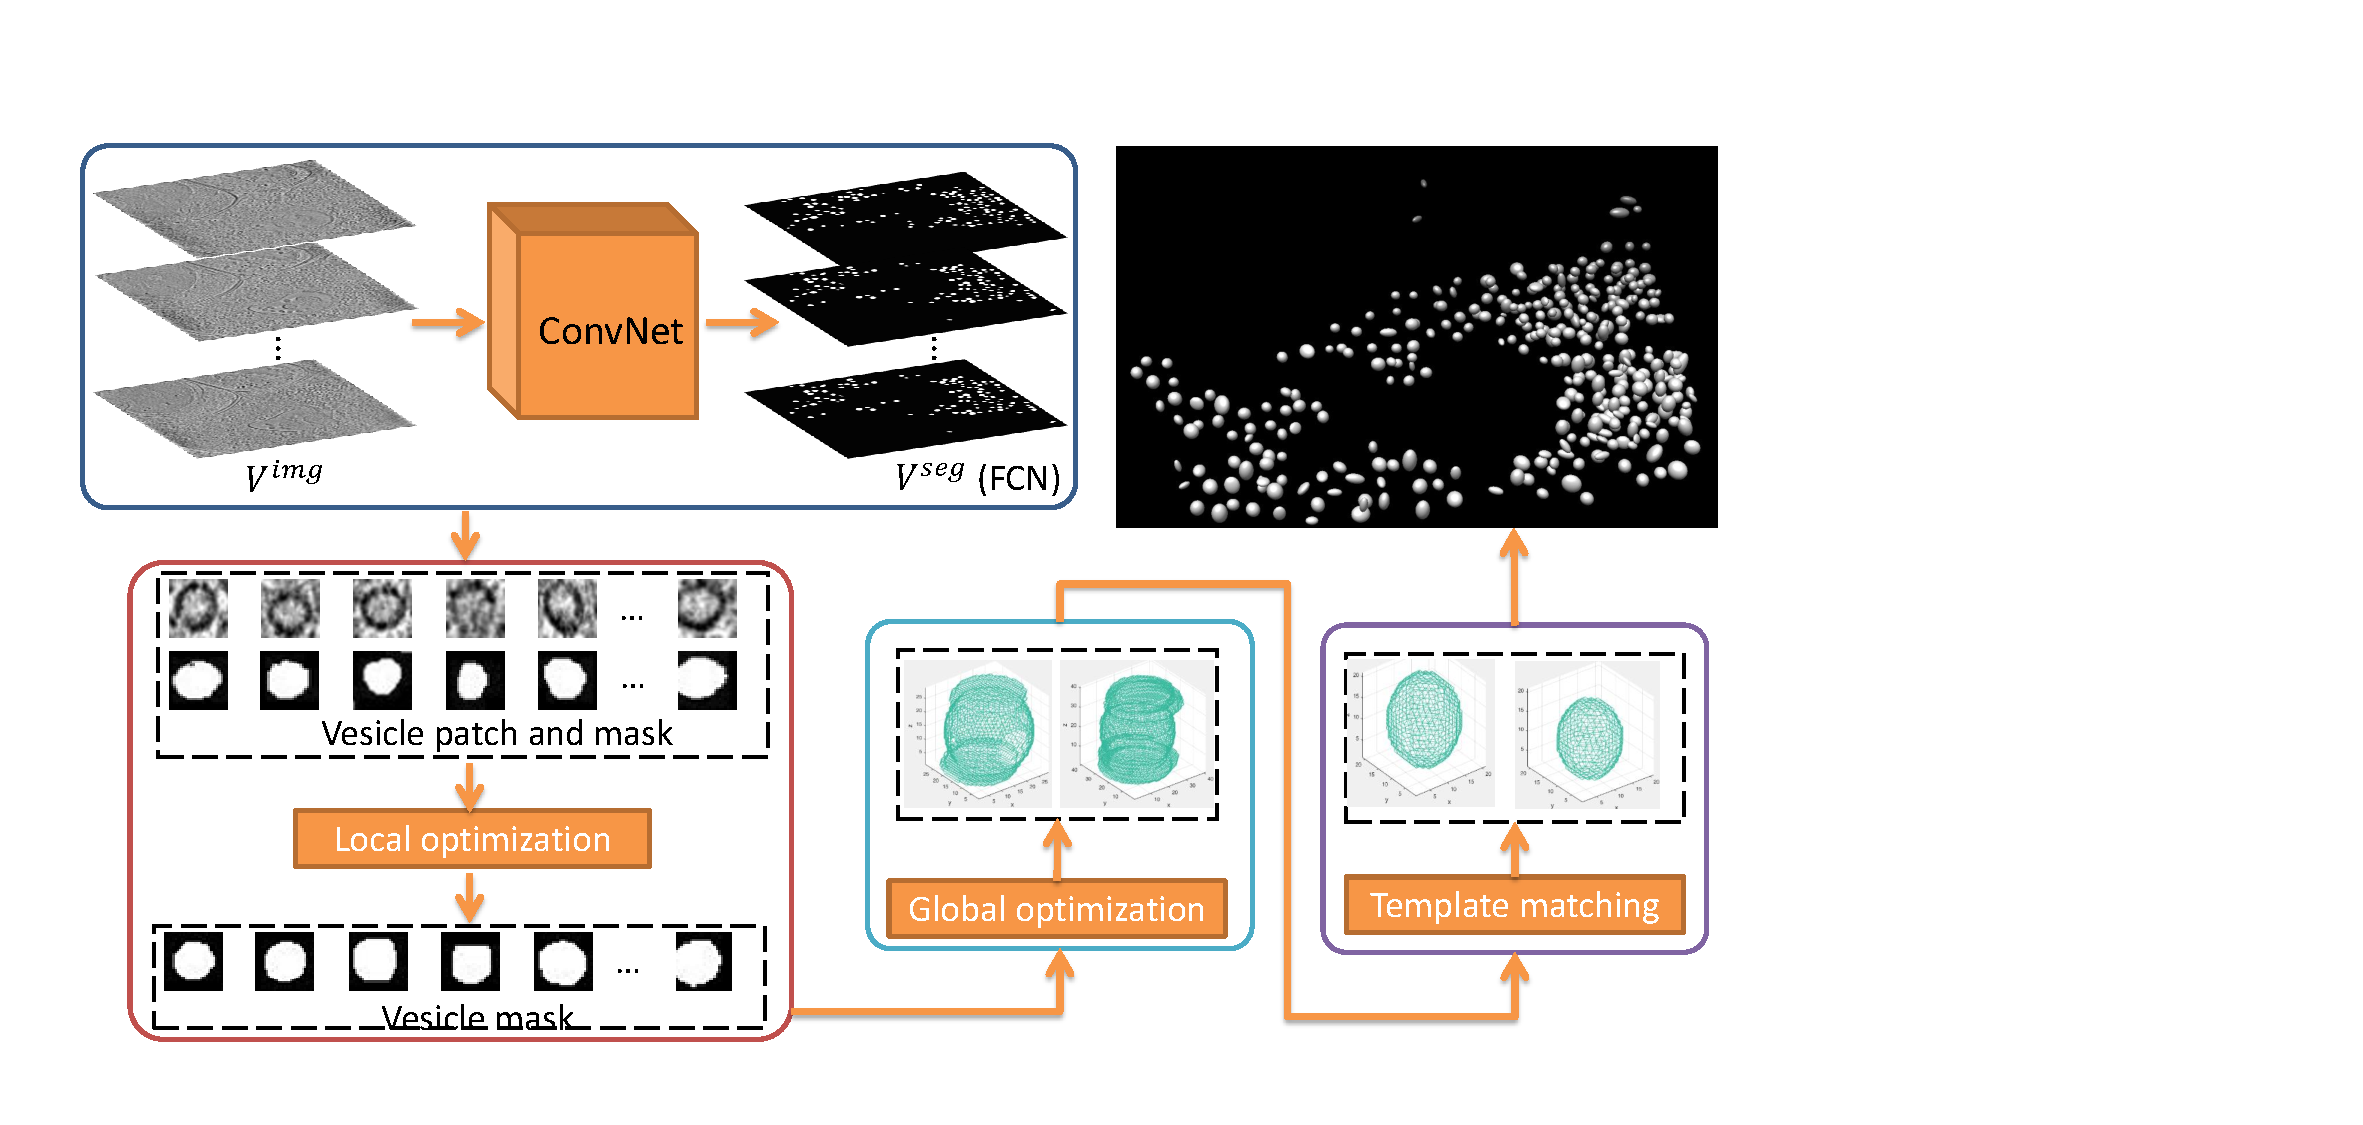
\includegraphics[width=6.7in]{figs/fig_pipline.pdf}
    \end{center}
    \caption{The diagrams of our framework. The orange arrows indicates the data flow, while the orange blocks denote our operation modules. It should be noted that local optimization refines 2D vesicle shapes in each image slice, and the global optimization refines the 3D shapes in the image volume.}
    \label{fig:pl}
\end{figure*}

To tackle the above challenges, we propose a novel system to automatically output the accurate shape description for each vesicle in a raw electron cryo-tomography data.
The whole pipeline is shown in Figure~\ref{fig:pl}, which mainly consists of four parts.
First, a convolution neural network is used to coarsely segment the vesicle region in $V^{img}$, and then two optimization strategies are developed to refine the vesicle shapes locally and globally.
Finally, a robust 3D vesicle matching algorithm is used to produce the undistorted 3D shapes of vesicles.

\subsection{Fully convolutional networks}
%For network architecture, we explore both performance of 3D and 2D FCNs. For 3D FCN, we use %the brand-new DenseVoxNet \cite{Yu2017} in our framework, which extends dense connection %architecture to 3D FCN and becomes the state-of-the-art method for 3D biomedical segmentation.
%\begin{eqnarray}\label{eq:FCN3}
%\begin{aligned}
%V^{seg}=f(V^{img})
%\end{aligned}
%\end{eqnarray}
%where $V^{seg}$ is the segmentation result, where label 1 indicates the vesicle region and %label 0 indicates the background region.
%$f$ is the segmentation function of FCN.
%As we only need to distinguish background and vesicle regions, its final classifier layer is %modified to be binary.

For network architecture, we use the famous DeepLab (ResNet-101) \cite{Chen2018}, which introduces the dilated convolution to enlarge the receptive fields of FCN without extra parameters.





And a binary classifier for two categories is also used. 
The final segmentation result is represented by:
\begin{eqnarray}\label{eq:FCN2}
\begin{aligned}
V^{seg}=stack(\{f(I_d)|d=1\ldots D\})
\end{aligned}
\end{eqnarray}
Where $I_d$ is the $d$-th image of $V^{img}$ and $f$ is the segmentation function of FCN.
$V^{seg}$ is the segmentation result, where label 1 indicates the vesicle region and label 0 indicates the background region.
Especially, 2D FCN has higher segmentation efficiency and a larger perception filed along $x-y$ plane, but the complementary information along $z$-axis is ignored.
In our experiments, we also compare our performance with the 3D FCN and analyse their performance.

It should be noted that $V^{seg}$ is usually noisy, because FCN is weak in localizing accurate contours, which requires low-level features of the input \cite{Chen2017}.
Especially, most vesicles in $V^{img}$ can be detected with a coarse region by FCN, but there still exists missing detection and the inaccurate contours problems, which are harmful to estimate accurate shapes
Next, we propose two optimization algorithms by respectively refining  $V^{seg}$ from local and global context information.

\subsection{Vesicle optimization in 2D image}
Define $S_d$ as $d$-th image of $V^{seg}$, and $v_{k,d}$ as the $k$-th vesicle in $S_d$, we first refine the contour of $v_{k,d}$ using local texture information in $S_d$ with our contour evolving algorithm.

Based on the traditional snake method \cite{Kass1988}, the closed contour of $v_{k,d}$ is represented by $\mathbf{v}(s)=(\mathbf{x}(s),\mathbf{y}(s))$, which is the initial contour.
Then, we attempt to minimize the following energy function by removing the initial contour:
\begin{eqnarray}\label{eq:Etotal}
E_{total} =&\int_{0}^{1} E_{int}\big( \mathbf{v}(s) \big)+ E_{ext}\big( \mathbf{v}(s)\big) ds \\\nonumber
E_{int} = & \alpha|\mathbf{v}^{'}(s)|^2+\beta|\mathbf{v}^{''}(s)|^2 \\
E_{ext} =& I\big( \mathbf{v}(s)\big) + \kappa G\big(\mathbf{v}(s)\big)\nonumber
\end{eqnarray}
where $\mathbf{v}^{'}(s)$ and $\mathbf{v}^{''}(s)$ are the first-order and second-order derivatives of $\mathbf{v}(s)$, controlling the cure to be smooth and flat.
$E_{ext}$ consists of a Gaussian smoothed image $I$ and a gradient magnitude map $G$, which drives the curve to the edge region with dark pixel values.
In order to obtain the optimal $\mathbf{v}(s)$, an iterative updating strategy is usually used by:
\begin{eqnarray}\label{eq:GVF}
\mathbf{x}_{t+1} = (A+\gamma I)^{-1}(\mathbf{x}_t-g_x(\mathbf{x}_t,\mathbf{y}_t))\\
\mathbf{y}_{t+1} = (A+\gamma I)^{-1}(\mathbf{y}_t-g_y(\mathbf{x}_t,\mathbf{y}_t))\nonumber
\end{eqnarray}
where $\mathbf{x},\mathbf{y}\in R^n$ are the coordinates of n sampling points on $\mathbf{v}(s)$. 
$A$ is the pentadiagonal banded matrix \cite{Kass1988}, and $\gamma$ is the step size.
$[g_x,g_y]$ are the gradients calculated on $E_{ext}$ respectively along $x$ and $y$.
Especially, the Gradient Vector Flow (GVF) algorithm \cite{Xu1998} is used to obtain a more robust $[g_x,g_y ]$.

However, the updating strategy of Eq.~\ref{eq:GVF} is much sensitive to the image noise, which is serious in our electron micrographs.
For examples, in some flat regions with small gradients, the external tension $E_{ext}$ is too weak to efficiently drive $\mathbf{v}(s)$ to the right region, which puts a high demand on the initial $v(s)$.
And some noisy regions may create gyrate $E_{ext}$, which trap the control points easily.
Finally, since $[g_x,g_y ]$ near the contours are usually over-large, the evolving points are easy to cross the optimal potions.

To this end, we design a new updating strategy for our task by:
\begin{eqnarray}\label{Eq:update}
\mathbf{x}_{t+1} = (A+\gamma I)^{-1}(\mathbf{x}_t+E_{ext}(\mathbf{x}_t,\mathbf{y}_t)\mathbf{n}_x)\\
\mathbf{y}_{t+1} = (A+\gamma I)^{-1}(\mathbf{y}_t+E_{ext}(\mathbf{x}_t,\mathbf{y}_t)\mathbf{n}_x)\nonumber
\end{eqnarray}
Where $\mathbf{n}_x,\mathbf{n}_y\in R^n$ are the normal vectors of n controlling points.
Especially, the directions of $\mathbf{n}_x,\mathbf{n}_y$ can be predefined, which in our task is from the inside out of vesicle.
Our Eq.~\ref{Eq:update} less depends on the initial $\mathbf{v}(s)$, because of the constant tensions of $\mathbf{n}_x,\mathbf{n}_y$ terms.
Different from the Ballons term in \cite{Cohen1991}, our constant tension is controlled by $E_{ext}(\mathbf{x}_t,\mathbf{y}_t)$, which means that, when $\mathbf{v}(s)$ is close to the optimal contour region, the evolving will become slow and finally stopping with a small $E_{ext}$.
And for the noisy images, our Eq.~\ref{Eq:update} is also more robust, because no gradients terms are used.
Figure~\ref{fig:lo} shows the evolving processing of different $E_{ext}(\mathbf{v}(s))$.
Experiments will demonstrate the effectiveness of our new updating strategy compared to commonly used GVF and Ballons in electron micrographs.

\begin{figure}
    \begin{center}
        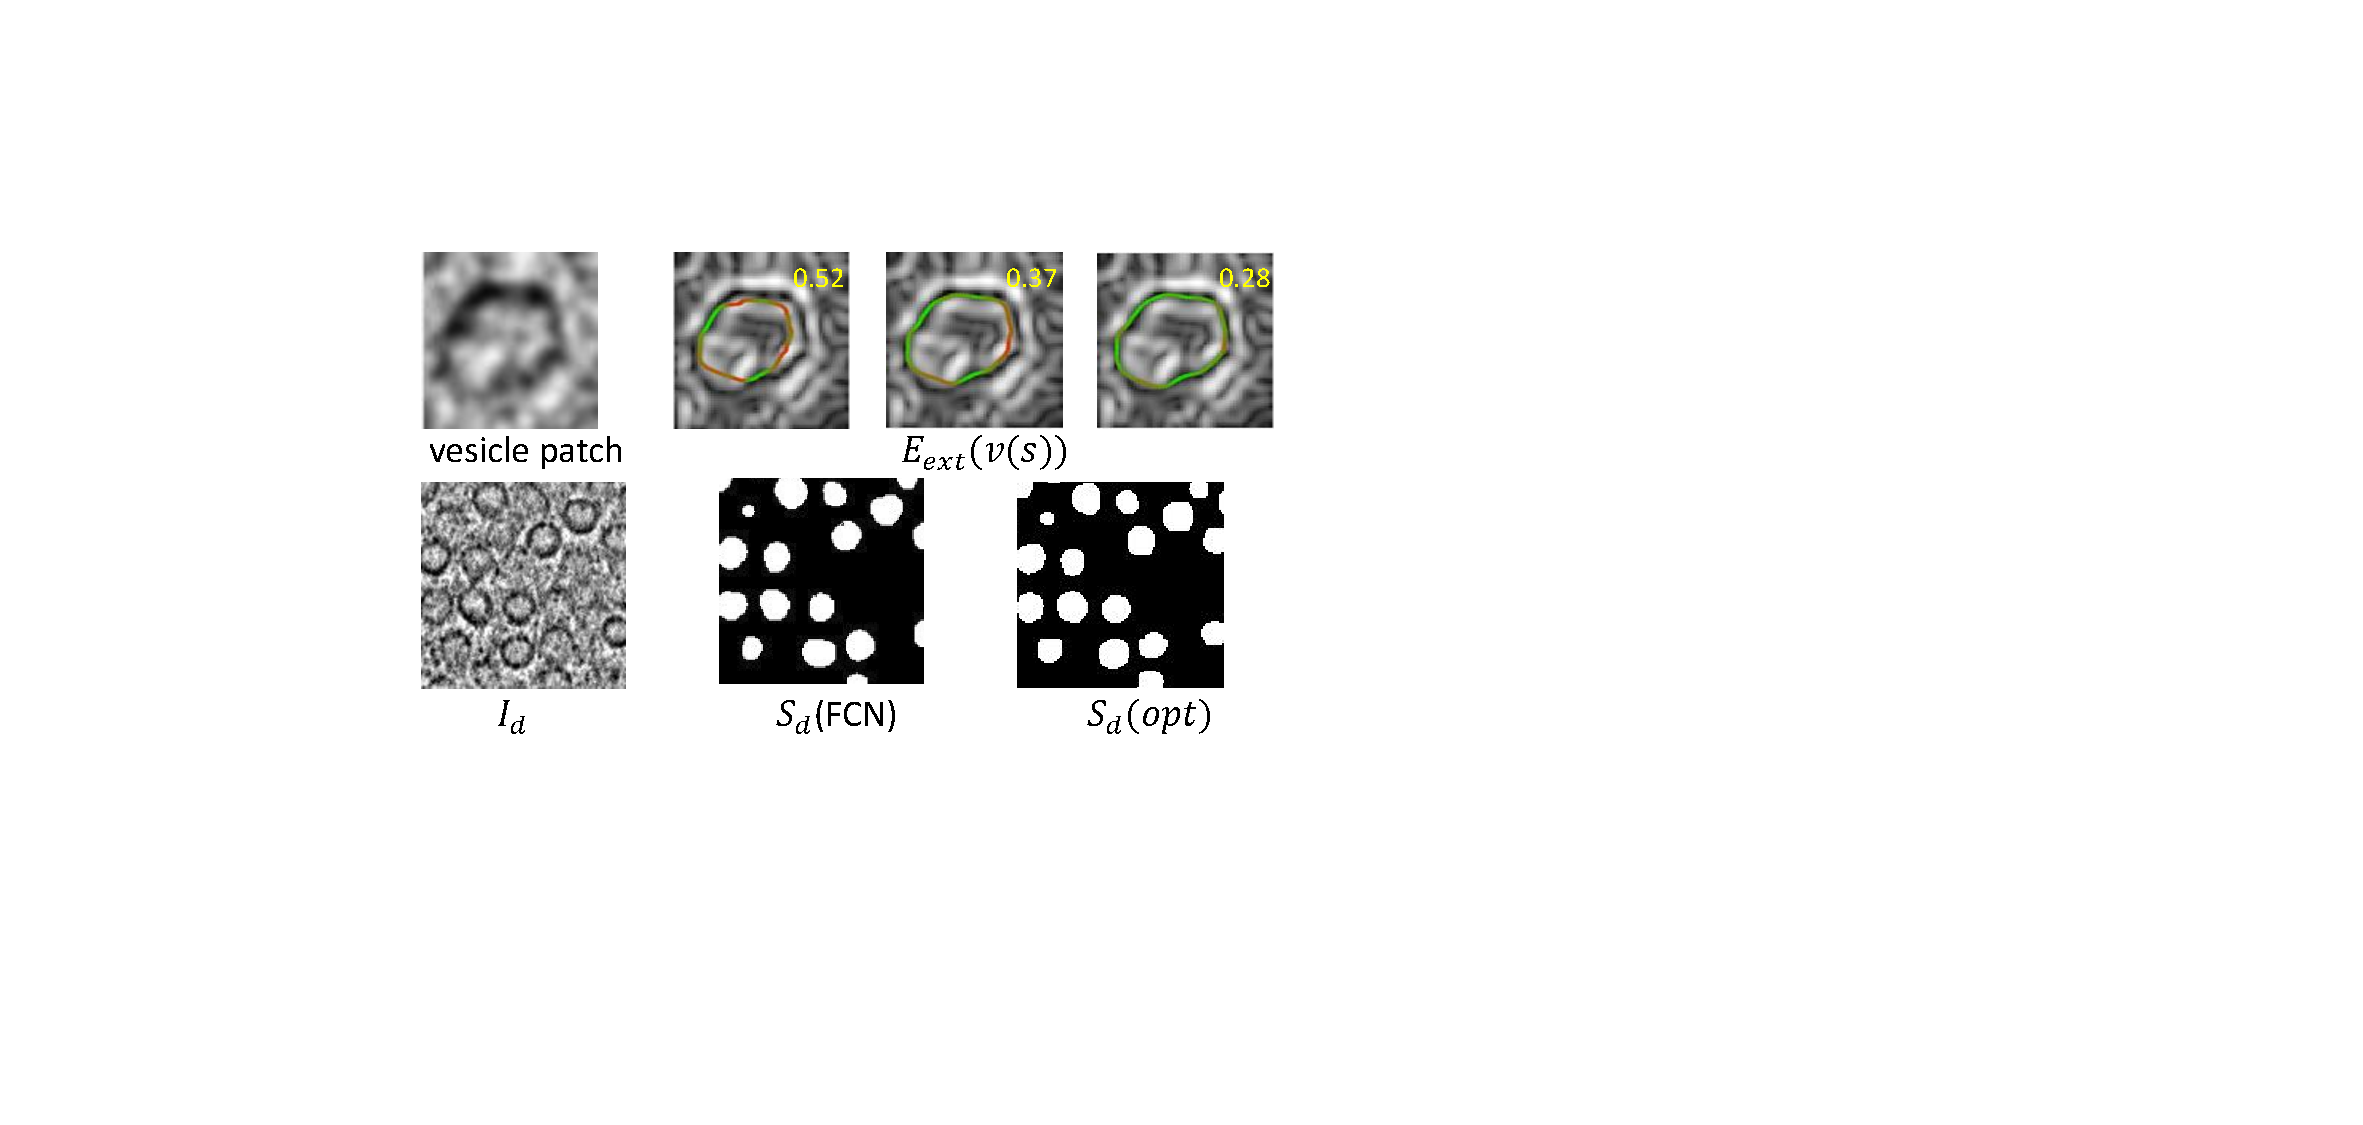
\includegraphics[width=3.3in]{figs/fig_lo.pdf}
    \end{center}
    \caption{At the top row, we visualize the evolving processing of Eq.~\ref{Eq:update}, by showing $E_{ext}$ and the $\mathbf{v}(s)$. Especially, the three images of $E_{ext}$ are respectively initial, middle and converge states. The yellow numbers are the value of $E_{ext}(\mathbf{v}(s))$, and the color of controlling points represents their $E_{ext}$ value. And the bottom row shows the an image patch with its segmentations (before and after local optimization).}
    \label{fig:lo}
\end{figure}

Finally, the optimal controlling points $[\mathbf{x},\mathbf{y}]$ from Eq.~\ref{Eq:update} make up a new curve $\mathbf{v}(s)$ as the optimized contour of $v_{k,d}$. 
After all $v_{k,d}$ have been refined with our contour evolving algorithm, the vesicle shapes in each $S_d$ are more accurate.

\subsection{ Vesicle optimization in 3D volume}
In this part, we develop a global association method, inspired by \cite{Xu2016,Zhang2008}, to solve the missing detection problem in $V^{seg}$ by FCN and associate vesicles in different $I_d$.
Especially, the method in \cite{Xu2016} will fail, when there exists missing detections in middle images of a vesicle.

Defining $n_d$ as the number of vesicles in the $d$-th image, our global association is modelled by:
\begin{eqnarray}\label{eq:go}
\min_{a_{i,j}}&\sum\limits_{i=1}^{n_{d1}}\sum\limits_{j=1}^{n_{d2}}a_{i,j}d(i,j)\hbar(d1,d2)\nonumber\\
s.t.& \sum\limits_{i=1}^{n_{d1}}a_{i,j}\leq 1, s.t. \sum\limits_{j=1}^{n_{d2}}a_{i,j}\leq 1\\
s.t.& \sum\limits_{i=1}^{n_{d1}}\sum\limits_{j=1}^{n_{d2}}a_{i,j}=min(n_{d1},n_{d2})\nonumber\\
s.t.& a_{i,j}\in \{0,1\}, d1<d2\nonumber
\end{eqnarray}
where $S_{d1}$ and $S_{d2}$ are any two images in $V^{seg}$.
$a_{i,j}$ is a binary variable of which 1 indicates $i$-th vesicle region on $S_{d1}$ and $j$-th vesicle region on $S_{d2}$ are connected and vice versa.
The conditions in Eq.~\ref{eq:go} constraint that each vesicle region in $S_{d1}$ has one associated region in $S_{d2}$ at most.
The $d(i,j)$ is the distance between $i$-th vesicle on $S_{d1}$ and $j$-th vesicle on $S_{d2}$ by:
\begin{eqnarray}\label{eq:d}
\begin{aligned}
d(i,j)&=\left\{\begin{array}{cc}
||C_{i,d1}-C_{j,d2}||_2^2&if v_{i,d1}\cap v_{j,d2}>0.8  \\
\infty & else\\
\end{array}\right.
\end{aligned}
\end{eqnarray}
where $C_{i,d}$ indicates the centroid of the $i$-the vesicle region in the $d$-th image.
In Eq.~\ref{eq:d}, if two vesicle regions have more than 80$\%$ overlapped region, we think they are overlapped.
And $\hbar(d1,d2)$ constraints that only $v_{i,d1}$ and $v_{j,d2}$ with close $d1$ and $d$ can be associated, by:
 \begin{eqnarray}\label{eq:hb}
\begin{aligned}
hbar(d1,d2)&=\left\{\begin{array}{cc}
1&if~d2-d1+1\leq \tau  \\
0 & else\\
\end{array}\right.
\end{aligned}
\end{eqnarray}
where $\tau$ controls the distance threshold of $d1$ and $d2$.

\begin{figure}
    \begin{center}
        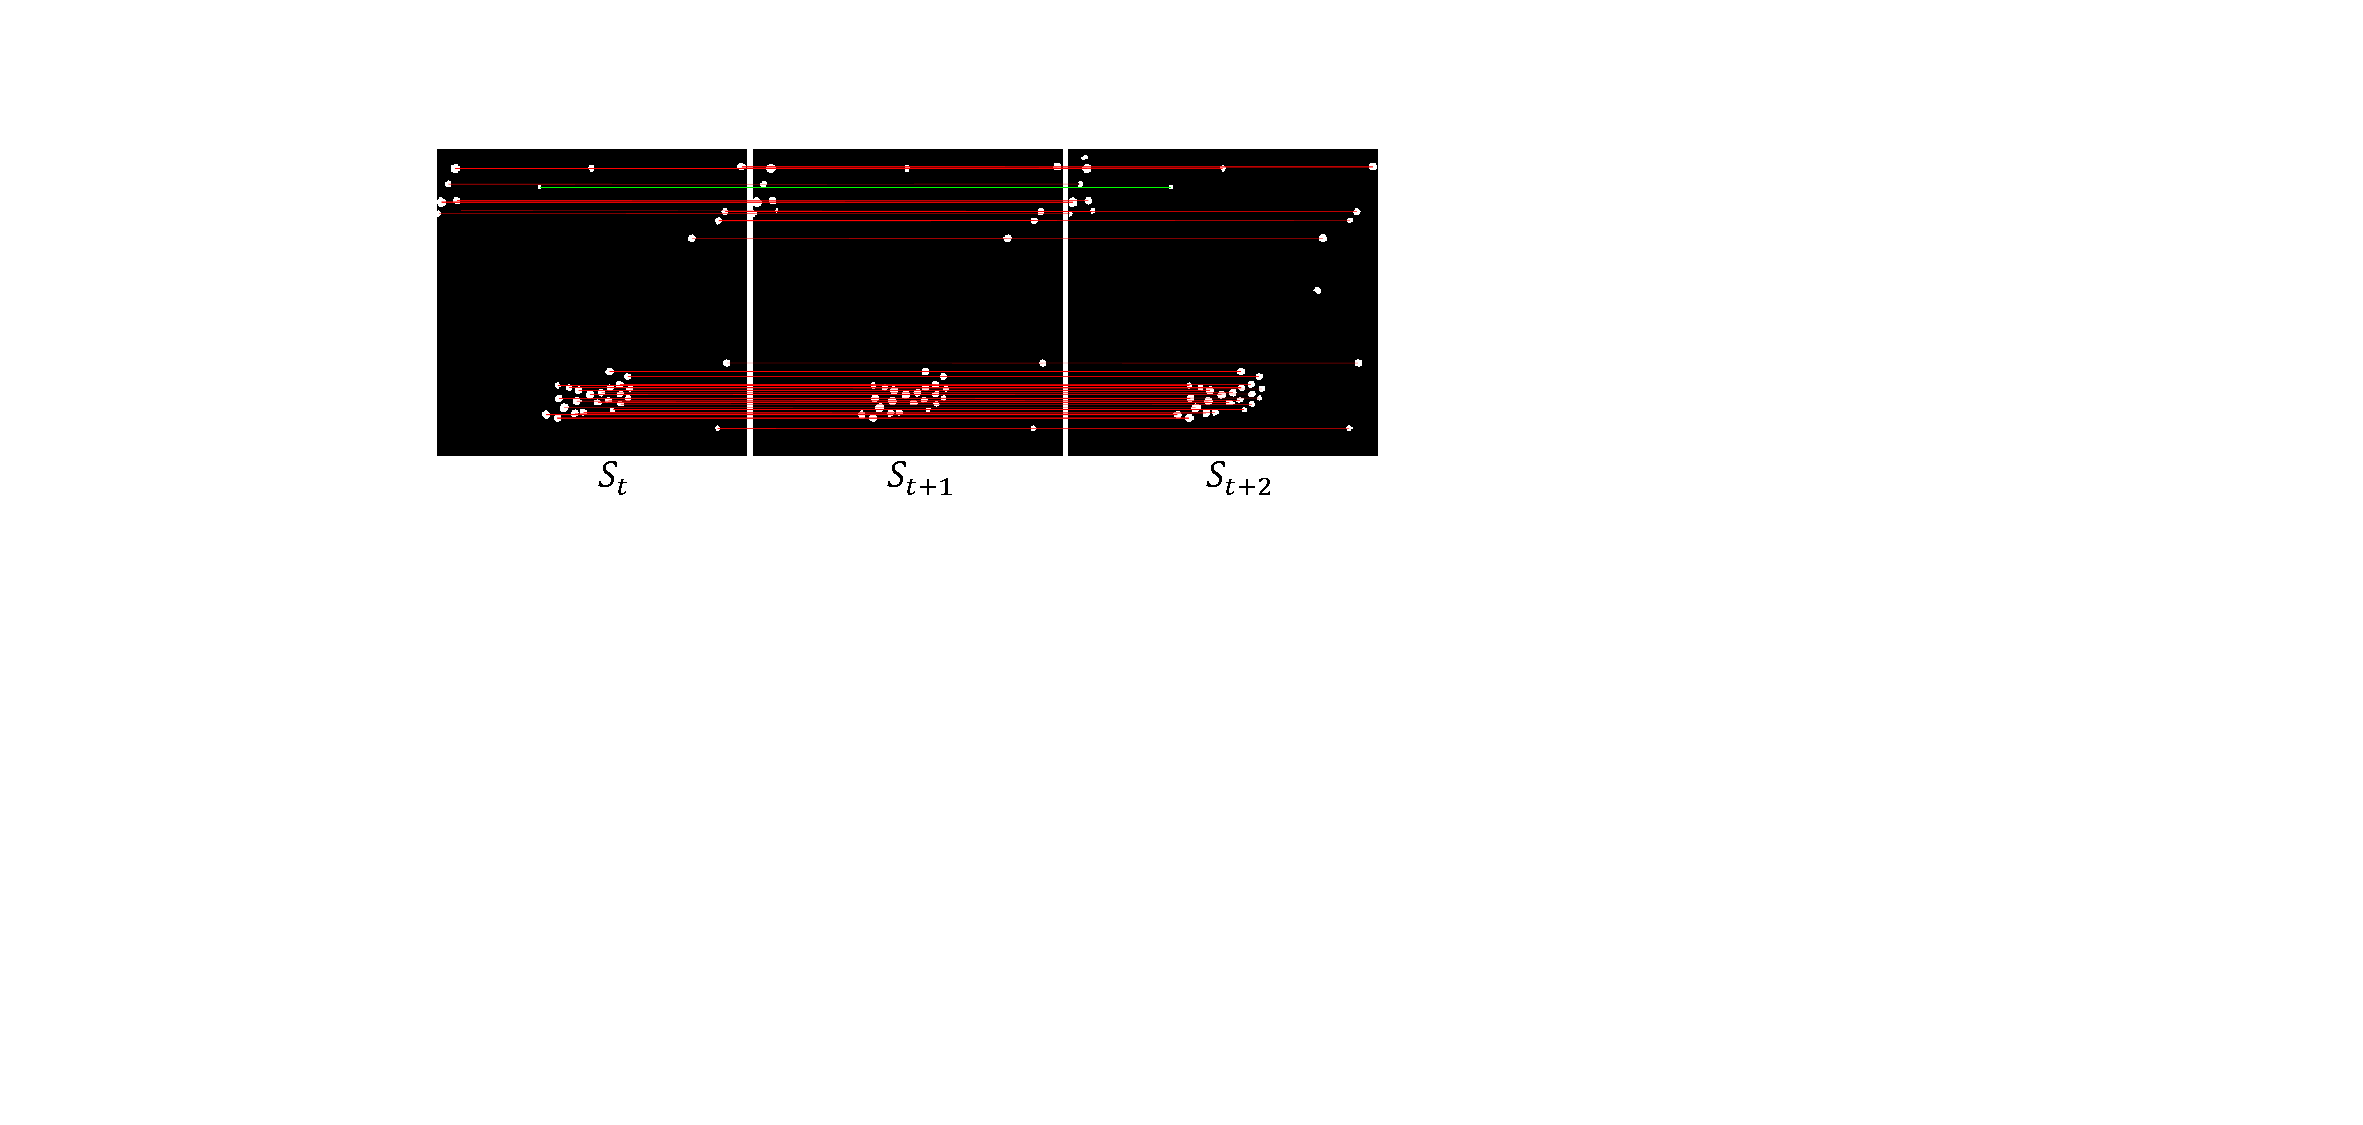
\includegraphics[width=3.3in]{figs/fig_go.pdf}
    \end{center}
    \caption{An example of global optimization. After optimization, vesicle regions belonging to the same vesicle have been well associated. And the green line indicates that our algorithm can associate two vesicle regions in two discontinuous slices, because of missing detection in middle slices, which is superior to \cite{Xu2016}.}
    \label{fig:go}
\end{figure}

Solving Eq.~\ref{eq:go} can not only associate continuous vesicle regions in adjacent images as one, but also associate discontinuous vesicle regions, as shown in Figure~\ref{fig:pl} (b).
The reason is that our $a_(i,j)$ is defined on and two images, which is different from \cite{Xu2016}, and a threshold function $\hbar(d_1,d_2)$ is proposed to control the acceptable number of discontinuous vesicle regions.
Specifically, when $\tau=1$, Eq.~\ref{eq:hb} degenerates to the method in \cite{Xu2016}, and when $\tau=\infty$, any vesicle regions with close $C$ will be associated.
And the Kuhn-Munkres algorithm \cite{Kuhn1955} is also used to solve the optimization for Eq.~\ref{eq:go}. 
Figure~\ref{fig:go} shows an example, which demonstrates the effectiveness of our algorithm.

\subsection{Vesicle template matching}
Now, we have the accurate segmentation $V^{seg}$ from FCN and our two-step optimizations.
The final part of our framework is to generate the vesicle description $p_i$ for each vesicle from $V^{seg}$, with the consideration of missing wedge problem.

Inspired by the method in [], we also use the template matching to recover the true shape of each vesicle.
Differently, our input is a binary volume, where 1 stands for vesicle region and 0 stands for background region, while the existing template matching based methods use the raw $V^{imgs}$ input.
Obviously, $V^{img}$ has much serious noisy texture than $V^{seg}$, and we can directly localize the vesicle positions in $V^{seg}$ for matching.
Therefore, our method is more accurate and efficient to generate $\{pi\}$ by matching.
 
Firstly, plenty of ellipsoids are generated to cover all shapes of vesicles, which make up a template collection $\Re={\omega_j |j=1\ldots N_t}$.
To reduce the matching space of $\Re$, we generate ellipsoids by sampling $[a_j,b_j,c_j]$ in [10,20] with the condition that at least one axis length equals $20$, and rotate them using different $\psi_i^{xy},\psi_i^z$ with step $20^{}\circ$.
Especially, the sampling density influences the matching accuracy and efficiency, which is a tradeoff.
Next, we make each $\omega_j$ distorted by simulating the imaging processing of $V^{img}$, of which the details is shown in supplementary materials.
Then, we have $\Re={(\omega_j,\hat{\omega}_j )|j=1\ldots N_t}$, where $\hat{\omega}_j$ is the distorted shape of $\omega_j$.
As all $v_{i,d}$ have been well associated in with global optimization, we can directly measure the similarity of a 3D vesicle shape $v_{i}$ in $V^{seg}$ and $\hat{\omega}_j$ by normalizing them to have the same maximum axis length.
Finally, we define that a similar $\hat{\omega}_j$ should have a large IoU with $v_{i}$ by:
\begin{eqnarray}\label{eq:iou}
IoU(v_i,\hat{\omega}_j) = \frac{v_i\cap\hat{\omega}_j}{v_i\cup\hat{\omega}_j}
\end{eqnarray}
where IoU indicates the fraction of intersection and union of $v_{i}$ and $\hat{\omega}_j$.

\begin{figure}
    \begin{center}
        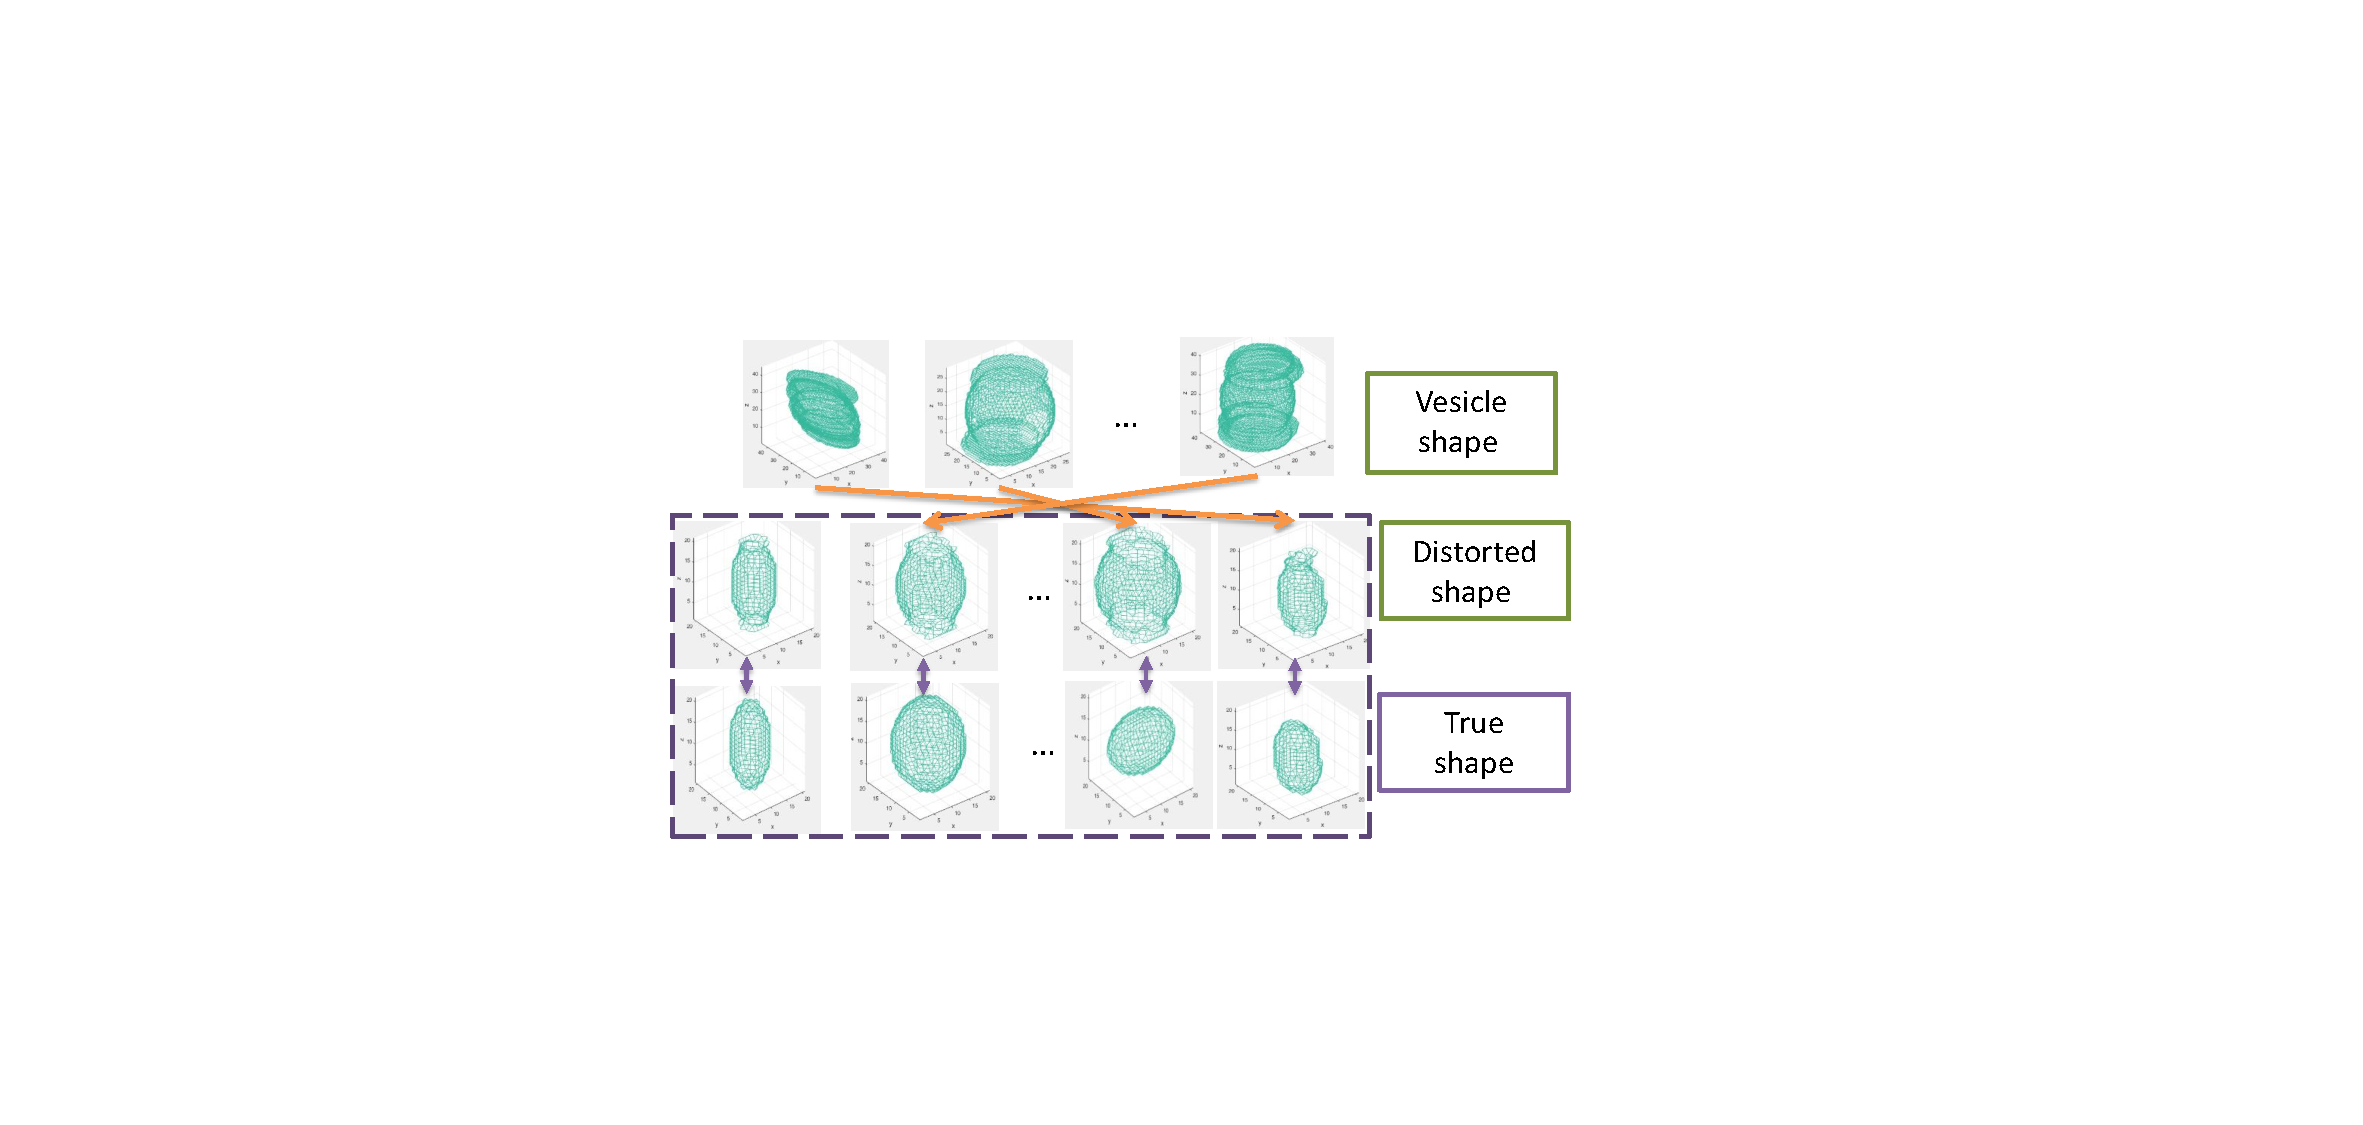
\includegraphics[width=3.3in]{figs/fig_tm.pdf}
    \end{center}
    \caption{A simple illustration of the template matching algorithm. The matching processing occurs between vesicle shapes and distorted templates, while the corresponding true templates are what we want. }
    \label{fig:tm}
\end{figure}

Solving Eq.~\ref{eq:iou}, we can assign a most similar $\hat{\omega}_j$ to each $v_i$, and the corresponding  $\omega_j$ is exactly the true shape of $i$-th vesicle.
Thus we can easily obtain the undistorted $p_i$ from $\omega_j$, whose shape parameters are known.
Figure~\ref{fig:tm} gives a simple diagram of the processing.

